\documentclass[lang=en,color=blue,mode=fancy,titlestyle=hang]{elegantbook}

% ---- Title Information ----
\title{Introduction to Compressed Sensing}
\author{Lancet Ross}
\date{Oct 15th, 2026}
\version{2.2}
\extrainfo{``What we know is not much. What we do not know is immense. --- P. S. Laplace''}

\cover{assets/3.1 What is Compressed Sensing/Compressed Sensing.png}

% ---- Additional Packages ----
\usepackage{amsmath}
\usepackage{array}
\usepackage{booktabs}
\usepackage{float}
\usepackage{wrapfig}
\usepackage{tabularx}
\usepackage{graphicx}
\usepackage{enumitem}
\usepackage{listings}
% Numbered captions are the house standard, so that \figref / \tabref resolve.
% The former \captionsetup[figure]{labelformat=empty} suppressed the "Figure N:"
% prefix and is deliberately not restored.
% Table of contents: body size throughout, opened up with leading.
\setlength{\cftbeforechapskip}{1.1em}
\setlength{\cftbeforesecskip}{0.5em}
\setlength{\cftbeforesubsecskip}{0.15em}
\usepackage{xcolor}
\usepackage{url}
\usepackage{xurl}
\usepackage{tikz}

% ---- Fonts ----
% The class loads ctex with fontset=none, so the CJK font must be set here.
% The tutorial is English, but it names the Chinese term 压缩感知 and cites one
% Chinese reference.
\usepackage{xeCJK}
\setCJKmainfont{Microsoft YaHei}
\setmonofont{Courier New}

% ---- Code listing style ----
\lstset{
  language=Matlab,
  basicstyle=\small\ttfamily,
  keywordstyle=\color{blue}\bfseries,
  commentstyle=\color{gray}\itshape,
  stringstyle=\color{orange},
  numbers=left,
  numberstyle=\tiny\color{gray},
  stepnumber=1,
  numbersep=8pt,
  showstringspaces=false,
  breaklines=true,
}

\begin{document}

\maketitle

\frontmatter
\tableofcontents

\mainmatter

\chapter*{Preface}
\addcontentsline{toc}{chapter}{Preface}

\linespread{1.55}\selectfont

Human beings have run into 21st century. The rapid development of information technology
has greatly increased the amount of data we need. It's clear that the real world is analog
and the digital world is discrete so that signal sampling is the necessary way to convert
the real world into the digital one. \textbf{Shannon-Nyquist sampling theorem} tells us
that the sampling rate should be at least twice the maximum frequency of the signal to
avoid aliasing, and this frequency is called the Nyquist frequency. However,
Shannon-Nyquist sampling theorem is faced with a problem that us humans wants to decrease
the cost of data sampling and storage. Is there a way to break through the
Shannon-Nyquist sampling theorem and sample the signal at a lower rate? The answer is yes,
and this is the \textbf{Compressed Sensing}.

We often call Compressed Sensing as CS for short, and also Compressive Sampling. Its
Chinese name is \textbf{压缩感知}, translated by Professor Qionghai Dai from Tsinghua
University. Compressed Sensing is a new theory that can reconstruct the original signal
from a small number of samples, which is much less than the Nyquist rate. For example, if
we lost \textbf{70\%} of the samples, we can still reconstruct the original signal with a
high probability. This is much unbelievable for us. Therefore someone said that Compressed
Sensing is the most important discovery in information theory since Shannon-Nyquist
sampling theorem.

To learn such a powerful theory is not easy. We need to start from the signal
transformation, and then some basic concepts like sparse representation and norm. The
final part is Compressed Sensing theory, we will introduce its concept and some
more like the observation matrices and the reconstruction algorithms. In this tutorial
we will mainly introduce greedy algorithms. I strongly recommended that you should have learned Teacher
Xue's \textbf{Signals and Systems} and \textbf{Linear Algebra} (no matter the teacher is 
Professor Liu or other teachers) before you start. 

Well, I was learning CS and writing this tutorial at the same time. Just like my last Linux
tutorial, I was writing it while I was at home. To be honest, I don't know much about CS,
and I even don't know if I can write this tutorial well. But I will try my best. If you find
any mistakes or have any suggestions, please feel free to contact me.

Let's rock and roll!

\begin{flushright}
  Lancet Ross\\
  Jul 24th, 2025
\end{flushright}

\linespread{1.2}\selectfont

\chapter{Signal Transformation}

\subsection*{Overview}

Compressed sensing rests on one observation: most signals are sparse in some domain, even
when they look dense in the one you started with. Finding that domain is the whole job of
this chapter, and everything that follows assumes you can name a transform in which your
signal has few significant coefficients.

We work through the two families that matter. The Fourier family covers the discrete
Fourier transform, its non-uniform variant, and the discrete cosine transform, while the
time-frequency family covers the short time Fourier transform and the continuous and
discrete wavelet transforms. The chapter closes with curvelets, which handle edges better
than wavelets do.

Every transform here follows the same pattern: a continuous version for the theory, a
discrete version you actually compute, and a fast algorithm for the discrete one, which
the chapter gives alongside the definition.


\section{Discrete Fourier Transform}

We have learned CTFT, CTFS, LT, DTFT and ZT in Signals and Systems. In this section
we will introduce the Discrete Fourier Transform (DFT).

\subsection{Definition}

The Discrete Fourier Transform (DFT) is created on the basis of the Discrete
Fourier Series (DFS). If we call a periodic signal $x_p(t)$, then we should notice
that it can't be two-side Z transformed, because it is not absolutely summable.
However, we can use the Discrete Fourier Series to represent it:
\[
  X_p(k) = \sum_{n=0}^{N-1} x_p(n)\,e^{-j\frac{2\pi}{N}kn},\quad k=0,1,\dots,N-1.
\]

And the inverse:
\[
  x_p(n) = \frac{1}{N}\sum_{k=0}^{N-1} X_p(k)\,e^{j\frac{2\pi}{N}kn},\quad n=0,1,
  \dots,N-1.
\]

For convience, we define that:
\[
  W = e^{-j\frac{2\pi}{N}}.
\]

Then we can rewrite the DFT and IDFT:
\[
  X(k) = \sum_{n=0}^{N-1} x(n)\,W^{kn},\quad k=0,1,\dots,N-1.
\]

\[
  x(n) = \frac{1}{N}\sum_{k=0}^{N-1} X(k)\,W^{-kn},\quad n=0,1,\dots,N-1.
\]

\subsection{Properties}

DFT processes discrete periodic signals. Its core is to periodic extend a finite
discrete sequence and still get a finite discrete sequence after DFT.

\subsubsection{Linearity}
\[
  DFT[a_1x_1(n) + a_2x_2(n)] = a_1DFT[x_1(n)] + a_2DFT[x_2(n)].
\]

\subsubsection{Shifting}
\textit{Firstly we need to notice two things:}

\textit{1. $x_p(n) = x((n))_N$ This means that $x_p(n)$ is a periodic signal with 
period $N$}

\textit{2. $x(n) = x_p(n)R_N(n) \quad R_N(n) = u(n) - u(n-N)$}

\textbf{Time shifting} is that if $y(n) = x((n-m))_NR_N(n)$ (This is called Circular
Shift m samples), then we have$Y(k) = W^{mk}X(k)$

\textbf{Frequency shifting} is that if $Y(k) = X((k-l))_NR_N(k)$, then we have
$y(n) = W^{-nl}x(n)$

\subsubsection{Circular Convolution}
In \textbf{time} domain if $y(n) = x(n)h(n)$ then we have:
\[
 Y(k) = \frac{1}{N}\sum_{n=0}^{N-1} X(l)H((k-l))_NR_N(k) = \frac{1}{N}\sum_{n=0}^{N-1}
H(l)X((k-l))_NR_N(k).
\]

In \textbf{frequency} domain if $Y(k) = X(k)H(k)$ then we have:
\[
  y(n) = \sum_{n=0}^{N-1} x(m)h((n-m))_NR_N(n) = \sum_{n=0}^{N-1} h(m)x((n-m))_NR_N(n).
\]

\subsubsection{Parseval's Theorem}
\[
  \sum_{n=0}^{N-1} |x(n)|^2 = \frac{1}{N}\sum_{k=0}^{N-1} |X(k)|^2.
\]

\subsubsection{DFT and ZT}
\[
  X(k) = X(z)|_{z=W^k}
\]

\[
  X(z)|_{z=e^{-j\frac{2\pi}{N}k}} = X(k)
\]

\subsection{Fast Fourier Transform}

The Fast Fourier Transform (FFT) is an algorithm to compute the DFT efficiently. The DFT
has a time complexity of $O(N^2)$, which is not efficient for large $N$. The FFT reduces
the time complexity to $O(N\log N)$ by exploiting the symmetries in the DFT.

Computers use FFT to compute the DFT, You can use fft() function in MATLAB, Python and
so on. \figref{fig:dft-fft-example} is a MATLAB example.

Here's an example of using FFT in MATLAB:
\begin{lstlisting}[language=Matlab]
L = 1500;               % length of signal
Fs = 1000;              % sampling frequency
S = 0.7*sin(2*pi*50*t) + sin(2*pi*120*t);
X = S + 2*randn(size(t));

% FFT and the single-sided spectrum
Y  = fft(X);
P2 = abs(Y/L);
P1 = P2(1:L/2+1);
P1(2:end-1) = 2*P1(2:end-1);

% frequency axis
f = Fs*(0:(L/2))/L;
\end{lstlisting}

\begin{figure}[htbp]
  \centering
  \includegraphics[width=0.9\textwidth]{assets/1.1 Discrete Fourier Transform/FFT
  Example.png}
  \caption{MATLAB FFT Example}
  \label{fig:dft-fft-example}
\end{figure}

\section{Non Uniform Fourier Transform}

\subsection{Definition}

FFT is fast, but also limited. The fact puts us into a dilemma: DFT requires that the
sampling points are uniformly distributed, but in real world the sampling points are not
always like this. So we have to find a way to deal with this problem. In this section we
will introduce the Non Uniform Fourier Transform (NUFT).

Let's take an example:

\begin{lstlisting}[language=Matlab]
t = sort([0:0.1:9.9, rand(1,20)*100]);
f = sin(2*pi*0.5*t) + 0.5*cos(2*pi*2*t);
\end{lstlisting}

This signal has 100 uniformly distributed sampling points and 100 non-uniformly ones,
How to solve this problem by NUFT?

\subsection{Process}

In fact, NUFT puts the non-uniformly distributed sampling points into uniformly
distributed ones, and then uses FFT. Academically speaking, NUFT uses convolution and
interpolation to reflect those sampling points into uniform grids. For example, above
200 sampling points can be distributed into (0,20) by every 0.1 seconds (according to
the size of interval and oversampling factor actually). Then use NUFFT.

\subsubsection{Kernel}
To interpolate sampling points, we introduce Kernel. Kernel is a function that
describes the shape of the interpolation.

\textbf{Gaussian Kernel} is a common kernel function, which is defined as:
\[
  \phi(x) = e^{-\frac{x^2}{2\sigma^2}}.
\]

$x$ is the distance from the sampling point to the grid point, and $\sigma$ is a width
parameter. Gaussian Kernel is simple that its accuracy and complexity grow with $\sigma$.

\textbf{Kaiser-Bessel Kernel (KB Kernel)} is another common kernel function, which is
defined as:
\[
  \phi(x) =
  \begin{cases}
    \dfrac{I_0\!\bigl(\beta\sqrt{1 - (2x/\omega)^2}\bigr)}{I_0(\beta)}, & |x|\le
    \tfrac{w}{2},\\ 0, & \text{otherwise},
  \end{cases}
\]

Here $I_0$ is the zero-order modified Bessel function, $\omega$ is the kernel’s support
width (typically 6–12), $\beta$ is the shape parameter given by
\[
  \beta = \pi\sqrt{\frac{w^2}{\alpha^2} - 0.5},
\]
and $\alpha$ is the oversampling factor (commonly 1.25, 1.5 or 2.0). The KB Kernel is
theoretically optimal and used in libraries such as FINUFFT, though its computation is
more involved.

\subsubsection{gridding}
The size of the grid equals to the oversampling factor times the original signal's size.
The steps of gridding are as follows: seek grid range, calculate the weight of kernel,
weighted accumulate to grid points, oversample the grid points.

\subsection{FINUFFT}

Things we talked above are the basic concepts of NUFT. There are many libraries
that can help us to do NUFT. For example the most famous one, \textbf{FINUFFT}.

FINUFFT is divided into three parts: finufft1d1, finufft1d2 and finufft1d3. They are
used to solve signals which are non-uniform in time domain, frequency domain and
both.

Here's a comparison of FINUFFT and FFT for a continuous signal, plotted in
\figref{fig:nuft-finuft-vs-fft}:
\begin{lstlisting}[language=Matlab]
fs = 1000;              % sampling frequency
L  = 1500;              % length of signal

% 1. Spread the uniform samples over [-pi, pi], as FINUFFT requires
t_uniform = (0:L-1)/fs;
T_total   = max(t_uniform) - min(t_uniform);
t_norm    = (t_uniform - min(t_uniform)) / T_total * 2*pi - pi;

x = 0.7*sin(2*pi*60*t_uniform) + sin(2*pi*120*t_uniform);

% 2. Compute the non-uniform transform in one call
ms = floor(L/2)+1;
Y  = finufft1d1(t_norm, x, -1, 1e-6, ms);
X  = abs(Y/L);
X  = X(1:floor(L/2)+1);
X(2:end-1) = 2*X(2:end-1);
f_target = (0:ms-1) * fs / L - fs/4;

% 3. Same spectrum by a plain FFT, for comparison
Y_fft = fft(x, L);
P1 = abs(Y_fft/L);
P1 = P1(1:floor(L/2)+1);
P1(2:end-1) = 2*P1(2:end-1);
\end{lstlisting}

\begin{figure}[htbp]
  \centering
  \includegraphics[width=0.95\textwidth]{assets/1.2 Non Uniform Fourier Transform/FINUFFT
  vs FFT.png}
  \caption{FINUFFT vs FFT}
  \label{fig:nuft-finuft-vs-fft}
\end{figure}

\section{Discrete Cosine Transform}

\subsection{Introduction}

Do you think such a question: Nature doesn't have many complex signals, most of the signals
are real. So why we use FT and create a complex basis function $e^{-j\omega t}$? Why not
just use cosine? Well this is what \textbf{Discrete Cosine Transform (DCT)} do.

\subsection{Definition}

DCT is a twice long DFT which for real even functions. Assume we have a right-side signal
$x(m)$, which is blue in \figref{fig:dct-process-1}. and we fold it back to the left side, which Is
the red part:

\begin{figure}[H]
  \centering
  \includegraphics[width=0.95\textwidth]{assets/1.3 Discrete Cosine Transform/DCT
  Process 1.png}
  \caption{DCT Process 1}
  \label{fig:dct-process-1}
\end{figure}

Now the new signal is not even, it has x=-0.5 as its symmetry axis. So we move it 0.5 to
the right, now it's even, as in \figref{fig:dct-process-2}:

\begin{figure}[htbp]
  \centering
  \includegraphics[width=0.95\textwidth]{assets/1.3 Discrete Cosine Transform/DCT
  Process 2.png}
  \caption{DCT Process 2}
  \label{fig:dct-process-2}
\end{figure}

Now DFT can be used to this signal:
\begin{align}
X(k) &= \sqrt{\frac{1}{2N}}\sum_{m'=-N+\tfrac12}^{N-\tfrac12} x\bigl(m'-\tfrac12\bigr)
        \cos\!\Bigl(\frac{2\pi m'n}{2N}\Bigr)\\
     &= \sqrt{\frac{2}{N}}\sum_{m'=\tfrac12}^{N-\tfrac12}x\bigl(m'-\tfrac12\bigr)
        \cos\!\Bigl(\frac{2\pi m'n}{2N}\Bigr)
        \quad(n = 0,1,\dots,N-1)
\end{align}

By replacing $m'$, we can obtain:
\[
  X(k) = \sqrt{\frac{2}{N}}\sum_{m=0}^{N-1} x(m)\cos\!\Bigl(\frac{(2m+1)n\pi}{2N}\Bigr)
  \quad(n = 0,1,\dots,N-1)
\]

However, now the DCT matrix is not orthogonal, so we need to normalize it:
\begin{align}
  X(k) &= a(n)\sum_{m=0}^{N-1} x(m)\cos\!\Bigl(\frac{(2m+1)n\pi}{2N}\Bigr)
  \quad(n = 0,1,\dots,N-1)\\
  a(n) &= \begin{cases}
    \sqrt{\frac{1}{N}}, & n = 0,\\
    \sqrt{\frac{2}{N}}, & n = 1,2,\dots,N-1.
  \end{cases}
\end{align}

This is the DCT, which is also called \textbf{DCT-II}, and IDCT is called \textbf{DCT-III}.
\begin{align}
  x(n) &= \beta(k)\sum_{k=0}^{N-1} X(k)\cos\!\Bigl(\frac{(2m+1)n\pi}{2N}\Bigr)
  \quad(m = 0,1,\dots,N-1)\\
  \beta(k) &= \begin{cases}
    \sqrt{\frac{1}{N}}, & m = 0,\\
    \sqrt{\frac{2}{N}}, & m = 1,2,\dots,N-1.
  \end{cases}
\end{align}

More than that, like FFT, DCT also has a fast algorithm called \textbf{Fast DCT (FDCT)}
with a time complexity of $O(NlogN)$. Its core is to break the DCT basis matrix into many
smaller matrices to reduce the calculation complexity.

\subsection{Application}

DCT is widely used in image and audio compression, such as \textbf{JPEG} and \textbf{MP3}.
It is especially effective for signals with a lot of low-frequency components, as it can
represent these components with fewer coefficients.


\section{Short Time Fourier Transform}

\subsection{Introduction}

Till now all we talked is in FT's field. FT is good, but not that good. It's a blind
method that can't tell us the time information of the signal. \figref{fig:stft-ft-disadvantage} is a proper example:

\begin{figure}[htbp]
  \centering
  \includegraphics[width=0.95\textwidth]{assets/1.4 Short Time Fourier Transform/FT's
  disadvantage.png}
  \caption{FT's disadvantage}
  \label{fig:stft-ft-disadvantage}
\end{figure}

If the blue signal is F1, the red one is F2, then F2 is the reverse of F1. But their
FTs are the same. It shows that FT can only find the frequency weight but can't tell
where the weight is.

It's also simple to solve this problem. Just divide the signal into two parts, the previous
second and the next second, do FT on both parts, and then we can get the time information.

This is called split by window in STFT. So there is a new concept called
\textbf{window function}.

\subsection{Definition}

STFT uses a window function to divide the signal into some parts, and then do FT on
each part. The core of STFT is to change the basis function to $e^{-j\omega t}y_{window}(t)$.

There are so many window functions, the most colorful one is the gate function $g_\tau(t)$
(This is also called Gabor Transform). All window functions are compact supported, which
means that they are non-zero only in a finite interval.

\subsection{Process}

We set the window function as $g_{0.5}(t)$ and $t_s$ is the time shift of it. Here's the
result of STFT:
\begin{lstlisting}[language=Matlab]
window_size = 0.5;          % width of the sliding window
ts          = [0.5, 1.0, 1.5, 2.0];   % window end times

for sig = 1:2               % X1 and X2
    for i = 1:length(ts)
        % 1. Cut one window out of the signal
        t_end   = ts(i);
        t_start = t_end - window_size;
        idx_start = find(t >= t_start, 1);
        idx_end   = find(t <= t_end, 1, 'last');
        segment   = X{sig}(idx_start:idx_end);
        seg_length = length(segment);
        % 2. FFT of that window
        Y  = fft(segment);
        P2 = abs(Y/seg_length);
        P1 = P2(1:floor(seg_length/2)+1);
        P1(2:end-1) = 2*P1(2:end-1);
        % 3. Plot it at height t_end
        f = Fs*(0:floor(seg_length/2))/seg_length;
        plot3(f, repmat(t_end, size(f)), P1, 'LineWidth', 2);
    end
end
\end{lstlisting}

The spectrum it produces is in \figref{fig:stft-example}.

\begin{figure}[htbp]
  \centering
  \includegraphics[width=0.95\textwidth]{assets/1.4 Short Time Fourier Transform/STFT
  Example.png}
  \caption{STFT Example}
  \label{fig:stft-example}
\end{figure}

STFT can distinguish the time information of the signal, every 0.5 seconds. When facing
more complex signals, we can use smaller window size to get more detailed time information.

\section{Continuous Wavelet Transform}

\subsection{Introduction}

Heisenberg Uncertainty Principle tells us that we can't get the time and frequency
information of a signal at the same time. The resolution of time and frequency domain
is always negative correlated. This means that if we want to get more detailed time
information, we have to sacrifice the frequency information, and vice versa.

For low frequency signals we hope to get higher frequency resolution, then the window
function will be wider. For high frequency signals we hope to get higher time
resolution, then the window function will be narrower.

It's certain that the time resolution will be lost to zero without window function. And
the window width of STFT is fixed, which means that its resolution is also fixed. This is
not good for us, because we want to get a varaible resolution. So we need a new window
function.

This is the \textbf{wavelet mother function}, shown in \figref{fig:cwt-mother-function}.

\begin{figure}[htbp]
  \centering
  \includegraphics[width=0.95\textwidth]{assets/1.5 Continuous Wavelet Transform/Wavelet
  mother function.png}
  \caption{Wavelet mother function}
  \label{fig:cwt-mother-function}
\end{figure}

\subsection{Definition}

Wavelet mother function is not a single function, but a family of functions. There are
4 conditions for a wavelet mother function:
\begin{enumerate}
  \item It should be a compact supported function.
  \item Its integral is zero.
  \item Admissibility condition: $\int_{-\infty}^{\infty} |\hat{\phi}(\omega)|^2
  \frac{d\omega}{\omega} < \infty$. Here $\hat{\phi}(\omega)$ is the FT of $\phi(t)$.
  \item Orthogonality condition: $\int_{-\infty}^{\infty} \phi(t) \phi(t - t_0) dt = 0$
  for $t_0 \neq 0$.
\end{enumerate}

The admissibility condition and orthogonality condition ensure that the wavelet transform
can be invertible.

The wavelet mother function has no fixed frequency but a range. Therefore, Wavelet Transform
is more like a Band Pass Filter (BPF).

Here's the \textbf{wavelet funtion}:
\[
  \psi^*(\tau,s) = \frac{1}{\sqrt{s}}\psi(\frac{t}{s}-\tau)
\]

It's very easy to understand. $\tau$ is the time shift, $s$ is the scale factor. $\frac{1}
{\sqrt{s}}$ is the normalization factor, which ensures that the energy is preserved.

When $s$ is small, the wavelet function is squezzed, which means that it has a high time
resolution. When $s$ is large, the wavelet function is stretched, which means that it has
a high frequency resolution. This is exactly what we want.

And Continuous Wavelet Transform (CWT) is similar to FT, which it just changes the basis
function to $\psi^*(\tau,s)$.

\subsection{Process}

See \figref{fig:cwt-example-1} and \figref{fig:cwt-example-2}$^{[1]}$. The yellow signal is the original signal, the blue one is the wavelet
function. \figref{fig:cwt-example-1} chooses a small $s$ to filter the high frequency part and \figref{fig:cwt-example-2}
chooses a large $s$ to filter the low frequency part. This is the idea of CWT.

\begin{figure}[htbp]
  \centering
  \includegraphics[width=0.75\textwidth]{assets/1.5 Continuous Wavelet Transform/CWT
  Example 1.png}
  \caption{A narrow wavelet $s=1$ slid across the signal$^{[1]}$}
  \label{fig:cwt-example-1}
\end{figure}
\begin{figure}[htbp]
  \centering
  \includegraphics[width=0.75\textwidth]{assets/1.5 Continuous Wavelet Transform/CWT
  Example 2.png}
  \caption{A wide wavelet $s=20$ slid across the signal$^{[1]}$}
  \label{fig:cwt-example-2}
\end{figure}

Teacher Xue said, no matter what kind of signal transformation it is, the core is the
basis function. All transformations perform inner product operation between the basis
function and the signal. FT's basis function is $e^{-j\omega t}$, which has no compact
support condition. STFT's basis function is $e^{-j\omega t}y_{window}(t)$, which a fixed
window width gives a fixed resolution. CWT's basis function is $\psi^*(\tau,s)$, which has
a variable window width and a variable resolution. That's why Wavelet Transform wins.

In the end, there are many wavelet mother functions, such as Haar wavelet, Daubechies
wavelet and so on. Use what kind of wavelet mother function depends on the signal
you want to process. It is always beneficial to refer to others' materials.

\section{Discrete Wavelet Transform}

\subsection{Introduction}

CWT solves the problem of STFT. However, CWT can only process continuous signals.
Like CTFT changes to DFT, CWT also has a discrete version, which is called DWT.
This is according to computer's discreteness and finiteness.

\subsection{Definition}

Mallat created a new algorithm to process DWT, which is called \textbf{Mallat Algorithm}.
The core of Mallat Algorithm is to use a pair of low-pass filter and high-pass filter
to decompose the signal into two parts: low frequency part and high frequency part.

Let the original signal pass through a LPF $h[n]$ and a HPF $g[n]$, if the highest
frequency of the signal is $\pi$, then the highest part(high frequency coefficient) is
($\pi/2, \pi$) and the lowest part is ($0, \pi/2$)(low frequency coefficient). This
process is called \textbf{half sub-band filtering}.

The process of diluting the sampling points by a factor of N is called N-fold
\textbf{subsampling}, on the other hand, the process of increasing the sampling points
by a factor of N is called N-fold \textbf{upsampling} (also called interpolation).

Both half sub-band filtering and 2-fold subsampling is called \textbf{wavelet decomposition}.

After first decomposition, now keep the high frequency coefficient and decompose the
low frequency coefficient twice, three times, and so on. Until it can't be
decomposed anymore (that is to say, 1).

Subsampling makes time resolution worse, but frequency resolution better. So we get our
result, variable resolution.

Here's the process$^{[1]}$ of Mallat Algorithm, drawn in \figref{fig:dwt-mallat-algorithm}:
\begin{figure}[htbp]
  \centering
  \includegraphics[width=0.7\textwidth]{assets/1.6 Discrete Wavelet Transform/Mallat
  Algorithm.png}
  \caption{Three-level filter bank of the Mallat algorithm$^{[1]}$}
  \label{fig:dwt-mallat-algorithm}
\end{figure}

\subsection{Example}

\begin{lstlisting}[language=Matlab]
wavelet = 'db4';        % db4 wavelet
level   = 4;            % 4 levels of decomposition

% 1. Multilevel decomposition, Mallat algorithm
[c, l] = wavedec(x_noisy, level, wavelet);

% 2. Pull the approximation and detail coefficients back out
A = cell(1, level);
D = cell(1, level);
for k = 1:level
    A{k} = wrcoef('a', c, l, wavelet, k);  % approximation at level k
    D{k} = wrcoef('d', c, l, wavelet, k);  % detail at level k
end

% 3. Reconstruct from the coefficients
x_recon = waverec(c, l, wavelet);
\end{lstlisting}

\begin{figure}[htbp]
  \centering
  \includegraphics[width=0.95\textwidth]{assets/1.6 Discrete Wavelet Transform/DWT
  Example.png}
  \caption{DWT Example}
  \label{fig:dwt-example}
\end{figure}

Approximation factor is the low frequency coefficient and detail factor is the high frequency
coefficient. Only D3 and D4 need to be retained, as the frequency components of the signal
are 50Hz and 100Hz. The error is extremely small, which shows the good performance of DWT.
The result is in \figref{fig:dwt-example}.

\section{Continuous Curvelet Transform$^{[7]}$}
\subsection{Introduction}

Similar to the Wavelet Transform, the Curvelet Transform is designed to represent data
with edges more effectively. It captures the directional information of curves in images,
making it particularly useful for image processing tasks.

\begin{figure}[htbp]
  \centering
  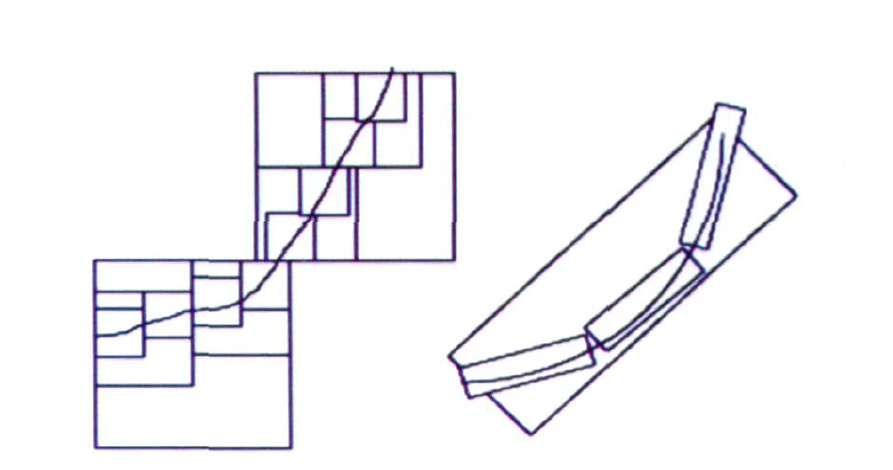
\includegraphics[width=0.95\textwidth]{assets/1.7 Continuous Curvelet Transform/WT and CT.png}
  \caption{WT (left) and CT (right) $^{[8]}$}
  \label{fig:cct-wt-vs-ct}
\end{figure}

Curvelet means small curves. when Curvelet Transform was invented, its aim was to replace
ridgelets, which are newer than wavelets. \figref{fig:cct-wt-vs-ct} puts a wavelet and a
curvelet side by side. Ridgelets are good at representing straight edges,
while curvelets excel at capturing curved edges. This makes curvelets particularly effective
for tasks involving images with complex structures and shapes.

The first generation of curvelets was constructed on the basis of the ridgelet transform.
However, too complex to implement so the second generation came out. Nowadays all we use
is the second generation.

\subsection{Definition}

Suppose in $R^2$, $x$ is the position parameter, $\omega$ is the frequency parameter,
$r, \theta$ are the polar coordinates. And there is $W(r), V(t)$ obeys:
\begin{align*}
  \sum_{j=-\infty}^{\infty} |W(2^{j}r)|^2 &= 1, \quad r \in (\frac34, \frac32) \\
  \sum_{l=-\infty}^{\infty} |V(t-l)|^2 &= 1, \quad t \in (-\frac12, \frac12)
\end{align*}

For any $j \geq j_0$, define:
\[
  U_j(r, \theta) = 2^{-\frac34 j}W(2^{-j}r)V(\frac{2^{[\frac{j}{2}]\theta}}{2\pi})
\]

$[\frac{j}{2}]$ means rounding down. The whole formula describes a wedge-shaped window,
drawn in \figref{fig:cct-tiling}:
\begin{figure}[htbp]
  \centering
  \includegraphics[width=0.6\textwidth]{assets/1.7 Continuous Curvelet Transform/Curvelet
  tiling of frequency.png}
  \caption{Curvelet tiling of frequency}
  \label{fig:cct-tiling}
\end{figure}

Let the mother curvelet be $\phi_j(\omega)$, and $\phi_j(\omega) = U_j(\omega)$. Also introduce:
\begin{itemize}
  \item rotation angles $\theta_l = 2\pi \cdot [\frac{j}{2}] \cdot l$ with $l = 0, 1, \ldots$
  such that $\theta_l \in \left[0, 2\pi\right)$.
  \item translation parameters $k = (k_1, k_2)$ with $k_1, k_2 \in Z^2$.
\end{itemize}

With this we define:
\[
  \phi_{j, k, l}(x) = \phi_j(R_{\theta_l}(x - x_k^{(j, l)}))
\]

Where we have:
\begin{align*}
  x_k^{(j, l)} &= R_{\theta_l}^{-1}(2^{-j}k_1, 2^{-\frac{j}{2}}k_2) \\
  R_{\theta_l} &= \begin{pmatrix}
    \cos\theta_l & -\sin\theta_l \\
    \sin\theta_l & \cos\theta_l
  \end{pmatrix}
\end{align*}

A curvelet coefficient is the inner product between $f$ and $\phi_{j, k, l}$:
\[
  c_{j, k, l} = \langle f, \phi_{j, k, l} \rangle = \int f(x) \phi_{j, k, l}(x) \, dx
\]

Also according to Plancherel's theorem, we have such formula in frequency domain:
\[
  c_{j, k, l} = \frac{1}{(2\pi)^2} \int \hat{f}(\omega) \hat{\phi}_{j, k, l}(\omega) \, d\omega
\]

\section{Discrete Curvelet Transform}
\subsection{Definition}

Just like the definition of the continuous curvelet transform, we define radius window
and angle window in Cartesian coordinates as:
\begin{align*}
  W_j(\omega) &= \sqrt{\Phi^2_{j+1}(\omega) - \Phi^2_{j}(\omega)} \\
  V_j(\omega) &= V(2^{[\frac{j}{2}]}\frac{\omega_2}{\omega_1})
\end{align*}

Where we have:
\[
  \Phi_j(\omega_1, \omega_2) = \phi(2^{-j}\omega_1)\phi(2^{-j}\omega_2)
\]

Also introduce 2 expressions:
\begin{align*}
  \tan \theta_l &= l \cdot 2^{[\frac{j}{2}]}, \quad l = -2^{[\frac{j}{2}]}, \ldots, 2^{[\frac{j}{2}] - 1} \\
  S_{\theta_l} &= \begin{bmatrix} 1 & 0 \\ \tan \theta_l & 1 \end{bmatrix}
\end{align*}

Now the Cartesian window can be described as, and
\figref{fig:dct-tiling-cartesian} shows the resulting tiling:
\[
  U_j(\omega) = W_j(\omega)V_j(S_{\theta_l}\omega)
\]

Here is what it looks like in Cartesian coordinates:
\begin{figure}[htbp]
  \centering
  \includegraphics[width=0.7\textwidth]{assets/1.8 Discrete Curvelet Transform/Curvelet
  tiling of frequency.png}
  \caption{Curvelet tiling of frequency in Cartesian}
  \label{fig:dct-tiling-cartesian}
\end{figure}

After a complex process (It wasn't given in paper actually :<), we can get the coefficient:
\[
  c_{j, k, l} = \int f(\omega) U_j(S^{-1}_{\theta_l}\omega) e^{i\langle S^{-T}_{\theta_l} b,
  \omega \rangle} \, d\omega
\]

\subsection{Fast Discrete Curvelet Transform}

Candès and others created a fast algorithm to compute the discrete curvelet transform,
which is called \textbf{Fast Discrete Curvelet Transform (FDCT)}.

There are 2 implementations of FDCT: \textbf{FDCT via Unequispaced FFT (FDCT-USFFT)} and
\textbf{FDCT via Wrapping (FDCT-Wrapping)}. The latter is more accurate and faster, so it's
widely used in practice.

It is very hard to understand without math background, so do I. But don't worry, authors
have provided the code in Matlab and C called \textbf{CurveLab}. You can download it
from \url{http://www.curvelet.org/}.

And there's also a README file in the code package, which is very helpful. Here I just
repeat some key files of 2d MATLAB warpping version:

\begin{itemize}
  \item fdct\_wrapping.m: forward curvelet transform.
  \item ifdct\_wrapping.m: inverse curvelet transform.
  \item fdct\_warpping\_param.m: returns the location of curvelets in phase-space.
  \item fdct\_wrapping\_dispcoef.m: returns a matrix of curvelet coefficients.
  \item fdct\_wrapping\_pos2idx.m: for a given scale and angle, returns the indices of
  curvelet closest to a given position.
  \item fdct\_wrapping\_demo\_basic.m: a basic demo of the curvelet transform.
  \item fdct\_wrapping\_demo\_denoise.m: a demo of image denoising using curvelets.
  \item fdct\_wrapping\_demo\_denoise\_enhanced.m: an enhanced demo of image denoising
  using curvelets.
\end{itemize}

\chapter{Basic Concepts}

\subsection*{Overview}

Chapter 1 gave us the transforms, and this chapter gives us the vocabulary to describe what
they produce. Three ideas carry most of the weight: sparsity, norms, and convex
optimization. If those are clear, the theory in Chapter 3 will read easily.

Sparsity is the property the whole field exploits, and it is defined by counting non-zero
entries in some basis. Norms give a way to measure size, and the chapter works through the
important ones, including why the $l_1$ norm behaves so differently from the $l_0$ "norm".
Convex optimization is the machinery that turns a sparse-recovery idea into something
solvable.

The rest of the chapter is applied: the projection matrix for building a measurement
system, and image quality assessment and BayesShrink for judging how good a reconstruction
is, both of which the later chapters rely on.


\section{Sparsity}

\subsection{Definition}

As we all know, Compressed Sensing is a typical problem of Machine Learning. So we need
to understand what sparsity is before starting.

Think a simple question: how to tell your friend in crowd? We just need to remember some
features of him, such as his face, height, clothes and so on. In fact the most common way
is to remember his face, because it's the most distinctive feature. There are so many
features on one's face, but we only need to remember a few of them. This is called
\textbf{sparsity}. Sparsity is a concept that describes the situation where only a few
elements in a vector are non-zero or significant, while the rest are zero or almost zero.

Except this, we also need to understand \textbf{overcompleteness}. Overcompleteness is a
concept that describes the situation where the number of features is greater than the
number of samples. In other words, overcompleteness means that using $m (m>>n)$ signals
to desribe a length $n$ signal. Overcomplete dictionary is quite normal in Machine Learning.

if $y$ is a signal, $D$ is a dictionary, and $\alpha$ is the coefficient matrix, then we have
such a formula:
\[
  y = D\alpha \quad s.t. \quad ||\alpha||_0 < \sigma.
\]

Every signal can be sparsity represented by an overcomplete dictionary. $s.t.$ is subject to.


\subsection{Application}

If we have a 1KB signal, we storage it in a $ 32 \times 32$ matrix. According to the sparsity
property of the signal, we can use a local $32 \times 64$ dictionary $D$ and a $64 \times
32$ coefficient matrix $\alpha$ to represent the signal. It's clear that $\alpha$ is sparse.
In terms of experience, there are 90\% of the elements in $\alpha$ are zeros. So only
$64 \times 32 \times 0.1 \approx 205$ effective elements in $\alpha$. We just need to
make a $205 \times 3$ matrix to store the effective elements and their positions (Coordinate,
COO, and matrix can be smaller if you choose Compressed Sparse Row, CSR). Sending that matrix
is all it takes, because the receiver can reconstruct the signal by $\alpha$ and $D$. In the
end, we only need to send 0.6KB to the receiver, which is much smaller than the original 1KB
signal.

Where does the saving come from? Not from a compression algorithm that runs after sampling.
The signal is sparse in the dictionary itself, and sparsity is what makes the reduction possible.

The 205 coefficients are all the receiver needs, together with their positions. The dictionary and
the basis behind it are design parameters known to both ends, so they never cost you bandwidth.

This is the difference between sampling and representing. A traditional system samples first and
compresses afterwards, so it pays for samples it will later throw away.

\section{Norm}

\subsection{Definition}

In mathematics, we often define a norm as a function that measures the size of a vector.
The $l_p$-norm of a vector $x$ is:
\[
  ||x||_p = \sqrt[p]{\sum_{i=1}^{n} |x_i|^p}.
\]

The most common norms are: \textbf{$l_0$-norm, $l_1$-norm and $l_2$-norm}.

$l_0$-norm is defined as the number of non-zero elements in the vector because the zero-time
root is not defined.

Most questions in Machine Learning (such as Compressed Sensing) hope to minimize the
$l_0$-norm. However, this is quite hard and almost unbelievable. So they choose another
way, which is to minimize the $l_1$-norm. The $l_1$-norm is defined as:
\[
  ||x||_1 = \sum_{i=1}^{n} |x_i|.
\]

$l_1$-norm is the sum of the absolute values of the elements in the vector. This kind
questions can be solved by \textbf{convex optimization}.

$l_2$-norm is defined as:
\[
  ||x||_2 = \sqrt{\sum_{i=1}^{n} |x_i|^2}.
\]

$l_2$-norm is also called \textbf{Euclidean norm}, which is the length of the vector.
It's widely used in the least squares method.

There is also a $l_{\infty}$-norm, which is defined as:
\[
  ||x||_{\infty} = \max(|x_1|, |x_2|, \ldots, |x_n|).
\]

$l_{\infty}$-norm is the maximum absolute value of the elements in the vector.It's widely
used in image processing.

\subsection{Overfitting and $l_1$-norm sparsity}

In machine learning, if the train set is too small, the model may fit the noise
in the train set, which is called \textbf{overfitting}. This means that the model
performs well on the train set but poorly on the test set. To avoid overfitting,
There is a way to add a $l_1$-norm regularization term to the loss function. Minimize
the $l_1$-norm and we can get a sparse solution, and avoid overfitting.

Here's an example$^{[2]}$ to understand why sparsity solves the overfitting problem.

\begin{note}
Suppose you are the king of a kingdom that has a large population and an OK overall GDP,
but the per capita is very low. Each one of your citizens is lazy and unproductive and
you are mad. Therefore you command “be productive, strong and hard working, or you die!”
And you enforce the same GDP as before. As a result, many people died due to your harshness,
those who survived your tyranny became really capable and productive.
\end{note}

The population is vector x, the command is the $l_1$-norm regularization term, and the
result is the sparse solution. \figref{fig:norm-lp-2d} draws the unit balls of $l_p$-norms.
The $l_1$-norm regularization term forces the model to
be sparse, which means those useless people die. Now everyone is productive.

But, why $l_1$-norm regularization term can make the model sparse? First we need to
understand what is look like$^{[3]}$ of $l_p$-norm in 2D space.

\begin{figure}[htbp]
  \centering
  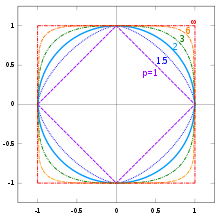
\includegraphics[width=0.6\textwidth]{assets/2.2 Norm/Lp-Norm in 2D space.png}
  \caption{$l_p$-norm in 2D space}
  \label{fig:norm-lp-2d}
\end{figure}

Take $l_1$-norm as an example, its intersection points with the coordinate axis are sparse
because there are zeros. We call these points as \textbf{sparse points}. Imagine that there
is a funtion, there are countless points on the function, once intersecting with the sparse
points of $l_1$-norm, $l_1$-norm determines the sparse solution on the function. So that's
why $l_1$-norm proves sparsity.

\section{Convex Optimization}

\subsection{Definition}

For arbitrary $x, y$ and $\mu \in [0, 1]$, then $\mu x + (1-\mu)y$ means all points
on the line segment between $x$ and $y$. If $x, y$ are in a set $C$ and $\mu x + (1-\mu)y$
is also in $C$, then $C$ is called a \textbf{convex set}. \figref{fig:convex-not-convex-set}
is a set that fails this test.

\begin{figure}[htbp]
  \centering
  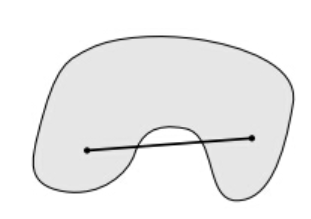
\includegraphics[width=0.4\textwidth]{assets/2.3 Convex Optimization/Not Convex Set.png}
  \caption{Not Convex Set}
  \label{fig:convex-not-convex-set}
\end{figure}

A function $f$ is called \textbf{convex function} if its domain is a convex set and for any
$x_1, x_2$ in the domain, the following inequality holds $f(\mu x_1 + (1-\mu)x_2) \leq \mu
 f(x_1) + (1-\mu)f(x_2)$, as \figref{fig:convex-function} illustrates.


If the inequality is strict, then $f$ is called a \textbf{strictly convex function}.

\begin{figure}[htbp]
  \centering
  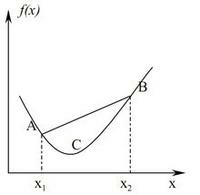
\includegraphics[width=0.4\textwidth]{assets/2.3 Convex Optimization/Convex Function.png}
  \caption{Convex Function}
  \label{fig:convex-function}
\end{figure}

If we have such an optimization problem
\[
  \min_{x} f(x)
  \quad\text{s.t.}\quad
  g_i(x)\le 0,\;i=1,2,\dots,l,
\]
and$f(x), g_i(x)$ are all convex functions, then this is called a \textbf{convex
optimization problem}.

\subsection{What's the usage?}

If a problem can be represented as a convex optimization problem, then it can be solved
much easier. This is because we have many algorithms to solve convex optimization problems.

There are some non-convex optimization problems, but convex optimization can play a
significant role in solving them. For example, Lagrange Relaxation Algorithm's non-convex
condition can be converted to convex.

For convex optimization problems, local optimal solution is also the global optimal solution.
This is because the convex function has no local minimum, which means that the local minimum
is also the global minimum. This is a very important property of convex optimization.

\section{Projection Matrix}

\subsection{Introduction}

If you have learned Prof.Liu's Linear Algebra, you must have watched Prof. Gilbert Strang's
video about Linear Algebra. In this section we will talk about the projection matrix in
his 16th lecture.

If there are 3 points, (1, 1), (2, 2) and (3, 2), and we want to find a line to fit these
points, then we get an equation:
\[
  \begin{array}{c@{\;\;}c@{\;\;}c@{\;\;}c}
    \begin{bmatrix}1 & 1 \\ 1 & 2 \\ 1 & 3\end{bmatrix}
    & \begin{bmatrix}C \\ D\end{bmatrix}
    & = & \begin{bmatrix}1 \\ 2 \\ 2\end{bmatrix} \\\\
    A & x & = & b
  \end{array}
\]

It's clear that there is no solution to this equation, so we choose the least squares method
to find the best solution:
\[
  x = (A^TA)^{-1}A^Tb.
\]

And this introduces \textbf{projection matrix}.

\subsection{Definition}

Actually, solve x is a process that use the linear combination of the column vectors of $A$
to approximate $b$. We set a vector $p$ which is the most close to $b$ and is in the
column space of $A$. Then the question becomes $\min ||b-p||_2$. and $p$ is called the
\textbf{orthogonal projection} of $b$ onto the column space of $A$.

We set $\hat{x}$ is the solution of the least squares method, then we have:
\[
  p = A\hat{x} = A(A^TA)^{-1}A^Tb = Pb.
\]

The matrix $P = A(A^TA)^{-1}A^T$ is called the \textbf{projection matrix}.

\subsection{Properties}

Projection matrices have several important properties:

\begin{itemize}
  \item Symmetry: $P^T = P$.
  \item Idempotence: $P^2 = P$.
  \item Eigenvalues are only 0 or 1.
  \item For any vector $b$, $Pb$ is the orthogonal projection of $b$ onto $Col(A)$, and the residual $r = b - Pb$ satisfies $r \perp Col(A)$.
  \item If $A = Q R$ is a full QR factorization with $Q^T Q = I$, then $P = Q Q^T$.
\end{itemize}

\subsection{Murmurs}

When I was writing this section, I realized that I had forgotten most of the knowledge about
Linear Algebra. I had to quick review it before I wrote almost everything. Study is a
process of forgetting and remembering. So I suggest you to review the knowledge
regularly, not only the required courses but also things like this tutorial. Well, after this
subsection, we will go into the most important part, \textbf{Compressed Sensing}. Hope you
can understand it well.

\section{Image Quality Assessment (IQA)}
\subsection{MSE and PSNR}

\textbf{Mean Squared Error (MSE)} is a basic metric for evaluating image quality. It
measures the average squared difference between the original image and the distorted
image. The formula is:
\[
  MSE = \frac{1}{mn} \sum_{i=0}^{m-1} \sum_{j=0}^{n-1} [I(i,j) - K(i,j)]^2
\]

$I$ is the original image, $K$ is the distorted image, and $m, n$ are the dimensions of
the images.

The image quality is better when MSE is smaller. However, MSE does not always align with
human visual perception. For example, a tiny loss in high-frequency details may result a
high MSE, but it may not be noticeable to human eyes.


\textbf{Peak Signal-to-Noise Ratio (PSNR)} is the most common metric for evaluating image
quality. It is derived from MSE and represents the ratio between the maximum possible
signal power and the noise power. The formula is:
\[
  PSNR = 10 \log_{10} \left( \frac{MAX_I^2}{MSE} \right) = 10 \log_{10} SNR
\]

where $MAX_I$ is the maximum possible pixel value of the image, which is $2^{bit depth} - 1$.
$MAX_I^{2}$ represents the maximum possible signal power.

When PSNR is higher, MSE will be lower, indicating the image quality is better. Generally,
a PSNR value above 30dB is considered acceptable for most applications. However, PSNR suffers
from the same limitations as MSE, it doesn't think about human sensitivity to different types
of distortions.

Though MSE and PSNR have their limitations, they are still widely used due to their simplicity
and ease of calculation. They provide a basic quantitative measure of image quality, but for
more comprehensive assessments, other metrics such as Structural Similarity Index (SSIM) are
often used.

\subsection{SSIM}

SSIM is an advanced metric, which is designed to better align with human visual perception.
It considers three key aspects of image quality: luminance, contrast, and structure.
\begin{itemize}
  \item Luminance: This measures the brightness of the image. The luminance comparison
  function is defined as:
  \[
    l(x,y) = \frac{2\mu_x \mu_y + C_1}{\mu_x^2 + \mu_y^2 + C_1}
  \]
  where $\mu_x$ and $\mu_y$ are the mean intensities of images $x$ and $y$, and $C_1$ is a
  small constant to avoid instability when the denominator is close to zero.

  \item Contrast: This measures the difference in intensity between pixels. The contrast
  comparison function is defined as:
  \[
    c(x,y) = \frac{2\sigma_x \sigma_y + C_2}{\sigma_x^2 + \sigma_y^2 + C_2}
  \]
  where $\sigma_x$ and $\sigma_y$ are the standard deviations of images $x$ and $y$, and
  $C_2$ is another small constant.

  \item Structure: This measures the correlation between the two images. The structure
  comparison function is defined as:
  \[
    s(x,y) = \frac{\sigma_{xy} + C_3}{\sigma_x \sigma_y + C_3}
  \]
  where $\sigma_{xy}$ is the covariance between images $x$ and $y$, and $C_3$ is a small
  constant.
\end{itemize}

$C$ is set to avoid instability when the denominator is close to zero, usually decided by
the dynamics of the image. The overall SSIM index is then calculated as:
\[
  SSIM(x,y) = [l(x,y)]^\alpha \cdot [c(x,y)]^\beta \cdot [s(x,y)]^\gamma
\]

To simplify, we usually set $\alpha = \beta = \gamma = 1$ and $C_3 = C_2/2$. So the formula
becomes:
\[
  SSIM(x,y) = \frac{(2\mu_x \mu_y + C_1)(2\sigma_{xy} + C_2)}{(\mu_x^2 + \mu_y^2 + C_1)
  (\sigma_x^2 + \sigma_y^2 + C_2)}
\]

SSIM values range from -1 to 1, where 1 indicates perfect similarity between the two images.

SSIM calculates a window (usually $11 \times 11$) to slide over the image, and
computes the SSIM index for each window. The final SSIM index for the entire image
is obtained by averaging the SSIM values of all windows.

\section{BayesShrink}
\subsection{Introduction}

To denoise a signal, we can use wavelet transform to transform the signal to wavelet
domain, then use a threshold to shrink the wavelet coefficients, and finally use inverse
wavelet transform to reconstruct the denoised signal.

There are many ways to choose the threshold, there are 2 common thresholds: \textbf{hard
threshold} and \textbf{soft threshold}.

Hard threshold means that if the absolute value of the wavelet coefficient is less than the
threshold, then set it to zero. Otherwise, keep it unchanged. The formula is:
\[
  D^H(U, \lambda) = \begin{cases}
    U, & |U| > \lambda \\
    0, & |U| \leq \lambda
  \end{cases}
\]

Soft threshold means that if the absolute value of the wavelet coefficient is less than the
threshold, then set it to zero. Otherwise, shrink it by the threshold. The formula is:
\[
  D^S(U, \lambda) = \begin{cases}
    sign(U)(|U| - \lambda), & |U| > \lambda \\
    0, & |U| \leq \lambda
  \end{cases}
\]

The most concerned thing is how to choose the threshold $\lambda$. A fixed universal threshold
is often used, which is defined as:
\[
  \lambda = \sigma \sqrt{2 \log n}
\]

where $\sigma$ is the noise level and $n$ is the number of wavelet coefficients.

However, this threshold is not adaptive to the signal, and may lead to problems. So that's
why \textbf{BayesShrink} comes out.

\subsection{BayesShrink}

The basic model of BayesShrink is:
\[
  Y = X + W
\]

where $Y$ is the observed signal, $X$ is the original signal, and $W$ is the noise. We
assume that $W \sim N(0, \sigma^2)$, and $X$ is independent of $W$.

The goal is to estimate $X$ from $Y$. BayesShrink finds a $T$ to make the MSE between $X$
and $\hat{X}$ minimum, where $\hat{X}$ is the estimated signal after thresholding.

And they also find that:
\[
  T = \frac{\sigma^2}{\sigma_X^2}
\]

$\sigma^2$ is the noise variance, and $\sigma_X^2$ is the variance of the original signal.

To estimate $\sigma^2$, we can use the HH1 subband of wavelet transform, because it is
mainly composed of noise.
\[
  \sigma^2 \approx \frac{1}{0.6745} median(|HH1|)
\]

To estimate $\sigma_X^2$, we can use the variance of the observed signal:
\[
  \sigma_Y^2 = \frac{1}{n} \sum_{i=1}^{n} Y_i^2
\]

Assume that noise and signal are independent, then we have:
\[
  \sigma_Y^2 = \sigma_X^2 + \sigma^2
\]

So we can get:
\[
  \sigma_X^2 = \max(\sigma_Y^2 - \sigma^2, 0)
\]

max is used to avoid negative values.

For a noisy image, we can follow such steps to denoise it:
\begin{itemize}
  \item Perform wavelet transform on the noisy image to get the wavelet coefficients.
  \item Estimate the noise variance $\sigma^2$ using the HH1 subband.
  \item For each subband, estimate the signal variance $\sigma_X^2$ using the wavelet
  coefficients.
  \item Calculate the threshold $T$ for each subband using $T = \frac{\sigma^2}{\sigma_X^2}$.
  \item Apply soft thresholding$^{[9]}$ to the wavelet coefficients using the calculated thresholds.
  \item Perform inverse wavelet transform to reconstruct the denoised image.
\end{itemize}

Moreover, if the standard deviation of the noise is known (Usually happens when the
noise is added to the signal), we can directly use its square as the noise variance
$\sigma^2$.

\chapter{Compressed Sensing}

\subsection*{Overview}

Now the theory itself, and the question is simple to state: if a signal is sparse in some
basis, how few measurements do we need in order to recover it exactly? The Nyquist rate is
the classical answer for band-limited signals, and compressed sensing shows that sparsity
buys us far more.

We start with the definition and the recovery condition. The restricted isometry property
is the key hypothesis, hard to verify but easy to reason about, and the chapter then covers
the observation matrices that satisfy it in practice, including random Gaussian and
Bernoulli matrices.

The last section is the algorithms. Greedy pursuit methods recover the signal one
coefficient at a time, starting with orthogonal matching pursuit and moving on to CoSaMP
and SAMP, which correct earlier mistakes and need less prior knowledge.


\section{What is Compressed Sensing?}

\subsection{Theoretical Framework}

Assume we have a $N$ long signal $X$, and $X$ can be sparsely represented by an orthogonal
basis $\Psi$, and we use an observation matrix $\Phi$ which is unrelated to $\Psi$, then We
get an observation signal $Y$, then reconstruct original signal $X$.

First, calculate the transformation factor $\Theta = \Psi^T$. Secondly, design an observation
matrix $\Phi$, then the observation signal $Y = \Psi \Theta = \Theta \Psi^T X$. Finally
this problem becomes a $l_0$-norm minimization problem:
\[
\min ||\Psi^T X||_0 \quad s.t. \quad Y = \Phi \Psi^T X.
\]

Compressed Sensing mainly includes three parts: signal's sparsity representation, observation
matrix design (also signal's low-speed sampling) and signal reconstruction.

\subsection{Signal's Sparsity Representation}

Under normal circumstances, we should choose specific basis $\Psi$, listed in
\tabref{tab:sparsity-bases}:

\begin{table}[H]
  \centering
  \begin{tabular}{|c|c|}
    \hline
    Application Scenario & Common Basis \\
    \hline
    1D signals      & Fourier basis, wavelets             \\
    Natural images  & DCT, wavelets, curvelets            \\
    ECG signals     & Wavelets                            \\
    Audio signals   & Gabor frames, Fourier basis         \\
    Video signals   & 3D DCT, wavelets                    \\
    MRI images      & Wavelets, curvelets                 \\
    \hline
  \end{tabular}
  \caption{Common bases for different application scenarios}
  \label{tab:sparsity-bases}
\end{table}

\subsection{Observation Matrix Design}

The core property of the observation matrix $\Phi$ is \textbf{Restrict Isometry (RIP)}.
RIP means that $\Phi$ can preserve the distance between the sparse signal and its
observation. In other words, $\Phi$ can ensure that the sparse signal can be reconstructed
from its observation. However, the RIP is very hard to satisfy, and there's an equivalent
conditions$^{[4]}$ for RIP: \textbf{Incorrectness between the observation matrix $\Phi$ and
the basis $\Psi$}. For most cases, \textbf{random Gaussian matrix} can satisfy this
condition. There are also some other matrices, we will show them soon.

Here's \figref{fig:cs-framework} to show Compressed Sensing$^{[5]}$, the observation matrix $\Phi$ is a
random Gaussian matrix, the basis $\Psi$ is a DCT basis.

\begin{figure}[htbp]
  \centering
  \includegraphics[width=0.95\textwidth]{assets/3.1 What is Compressed Sensing/Compressed
  Sensing.png}
  \caption{Compressed Sensing}
  \label{fig:cs-framework}
\end{figure}

\subsection{Signal Reconstruction}

We have talked that Compressed Sensing can be transformed to a $l_1$-norm minimization
problem, and this is a convex optimization problem ($l_1$-norm is convex and the equation
is also convex). There are three kinds of methods to solve this problem: \textbf{Convex Relaxation
Method}, \textbf{Greedy Pursuit Method} and \textbf{Iterative Thresholding Method}.

The typical representative of convex relaxation method is \textbf{Basic Pursuit (BP)},
\textbf{Basic Pursuit Denoising (BPDN)}, while greedy pursuit method is \textbf{Orthogonal
Matching Pursuit (OMP)} and \textbf{Compressive Sampling Matching Pursuit (CoSaMP)}. 
Iterative thresholding method is \textbf{Iterative Hard Thresholding (IHT)} and
\textbf{Iterative Soft Thresholding (IST)}. Every Algorithm has its own advantages and
disadvantages, and the choice of algorithm depends on the specific application scenario.
We will discuss greedy pursuit method in this tutorial.

\section{Common Observation Matrices}

\subsection{Random Gaussian Matrix}

Random Guassian Matrix is the most commonly used observation matrix in Compressed Sensing.
Make a $M \times N$ matrix $\Phi$, and every elements obey Gaussian distribution
$N (0,\frac{1}{M})$. That is to say:
\[
  \Phi_{ij} \sim N(0, \frac{1}{M}).
\]

This matrix has a high probability of meeting the RIP condition, and need not very large
measurements.

Here's a simple example in MATLAB:

\begin{lstlisting}[language=Matlab]
%% Random Gaussian Matrix Example
Phi = randn(M, N) / sqrt(M);
\end{lstlisting}

\subsection{Random Bernoulli Matrix}

Random Bernoulli Matrix is a special case of random Gaussian matrix. It is a $M \times N$
matrix, and every elements obey Bernoulli distribution:
\[
  \Phi_{ij} = \frac{1}{\sqrt{M}}
  \begin{cases}
    +1 \quad P=\tfrac12 \\
    -1 \quad P=\tfrac12
  \end{cases}
  \text{or} \quad
  \Phi_{ij} = \frac{3}{\sqrt{M}}
  \begin{cases}
    +1 \quad P=\tfrac16 \\
    0 \quad P=\tfrac23 \\
    -1 \quad P=\tfrac16
  \end{cases}
\]

This matrix is more convient to storage and transmission than random Gaussian matrix.

Here's a simple example in MATLAB:

\begin{lstlisting}[language=Matlab]
%% Random Bernoulli Matrix Example
Phi = randi([0, 1], M, N)
Phi(Phi == 0) = -1;
Phi = Phi / sqrt(M);
\end{lstlisting}

\subsection{Sparse Random Measurement Matrix}

Make an all-zero $M \times N (M < N)$ matrix $\Phi$, randomly choose $d (d < M)$ positions in each
columns and set them to 1. There isn't much difference when $d = \{4, 8, 10, 16\}$. This matrix
is also easy to storage.

Here's a simple example in MATLAB:

\begin{lstlisting}[language=Matlab]
%% Sparse Random Measurement Matrix Example
Phi = zeros(M, N);
for i = 1:N
    idx = randperm(M, d);
    Phi(idx, i) = 1;
end
\end{lstlisting}

\subsection{Toeplitz Matrix}

We define a Toeplitz matrix as:
\[
  T = \begin{bmatrix}
    t_n & t_{n-1} & \cdots & t_1 \\
    t_{n+1} & t_n & \cdots & t_2 \\
    \vdots & \vdots & \ddots & \vdots \\
    t_{2n-1} & t_{2n-2} & \cdots & t_n
  \end{bmatrix}
\]

When we construct a Toeplitz matrix, set a random vector $u = (u_1, u_2, \ldots, u_n)$ and
do a $M (M < N)$ times loop to construct $M-1$ rows. Then normalize the matrix at last.
Usually the value of $u$ is $\pm 1$ and obey Bernoulli distribution like random Bernoulli
matrix. In practice, the application prospects of T-matrix are relatively good because
cyclic displacement is easy to implement in hardware.

Here's a simple example in MATLAB:

\begin{lstlisting}[language=Matlab]
%% Toeplitz Matrix Example
u = randi([0, 1], 1, 2*N-1);
u(u == 0) = -1;

Phi = toeplitz(u(N:end), fliplr(u(1:N)));
Phi = Phi(1:M, :);
\end{lstlisting}

\section{Greedy Pursuit Method}

\subsection{Introduction}

When $A$ and $x$ are known, it's easy to solve $y = Ax$. But if $A$ and $y$ is known,
how to calculate $x$?

A way is that $x = A^{-1}y$, but we know the inverse matrix is hard to calculate,
and the matrix $A$ may not be invertible. So we need a new way to solve this problem.
This is the original idea of Matching Pursuit (MP).

However, MP has many problems, to solve these problems, a very important algorithm
called \textbf{Orthogonal Matching Pursuit (OMP)} was proposed. OMP is a typical greedy
pursuit algorithm, In this section, we will introduce OMP and its variants.

\subsubsection[\textbf{Examples}]{\textbf{Examples}\textsuperscript{[6]}}

\subsubsection{Example 1}
\[
  y = \begin{bmatrix} 1.65 \\ -0.25 \end{bmatrix}, \quad
  A = \begin{bmatrix} -0.707 & 0.8 & 0 \\ 0.707 & 0.6 & -1 \end{bmatrix}
\]

$A$ can be represented as a set of column vectors, and these vectors are called
\textbf{atoms}. The goal of OMP is to find a linear combination of these atoms to
reconstruct $y$. So we need to find which atom contributes to $y$ most, and which
second, and so on. This process iterates N times, where N is the number of atoms.
In this example, N = 3.

Contribution $\omega_i$ is $|<b_i, y>|$ or $|b_i^Ty|$. In this example, we have:
\[
  \omega = \begin{bmatrix}
    |<b_1, y>| \\
    |<b_2, y>| \\
    |<b_3, y>|
  \end{bmatrix}
  = \begin{bmatrix}
    |-1.34| \\
    |1.17| \\
    |0.25|
  \end{bmatrix}
\]

So we choose $b_1$ as the first atom, write it into a new matrix $A_{new}$, then
calculate residual $r = y - b_1\omega_1 = \begin{bmatrix} 0.7 \\ 0.7 \end{bmatrix}$.
Also, create a contribution matrix $x_{rec} = \begin{bmatrix} -1.34 \\ 0 \\ 0
\end{bmatrix}$ to record the contribution of $A_{new}$ to $y$ \textbf{(Not $\omega$!)}.

Actually, every time we calculate $x_{rec}$, least squares method is needed.
Because $b_i$ is normalized ($l_1$-norm is 1) in this example, we can use $w_i$ for
the first time. We will talk about this later.

Then we repeat this process, calculate the contribution of $b_2$ and $b_3$ to $r$,
and choose $b_2$ as the second atom, write it into $A_{new}$, and calculate $x_{rec}$.

To calculate $x_{rec}$, we need to calculate $\lambda$ that makes $\sum \lambda_i b_i$
most close to $y$. This is a least squares problem, like following equation:
\[
  \min ||A_{new} \cdot \lambda - y||_2
\]

The solution is:
\[
  \lambda = (A_{new}^TA_{new})^{-1}A_{new}^Ty.
\]

And sometimes QR decomposition is used to solve this equation, which is more stable.
\[
  A_{new} = QR \Rightarrow \lambda = R^{-1}Q^Ty.
\]

Upon completing this, we have $x_{rec} = \begin{bmatrix} -1.2 \\ 1 \\ 0 \end{bmatrix}$,
now $r = y - A_{new} \cdot \lambda = \begin{bmatrix} 0 \\ 0 \end{bmatrix}$.  This is the
answer.

\subsubsection{Example 2}
\[
  y = \begin{bmatrix} 2.7 \\ 0.1 \\ 4.5\end{bmatrix}, \quad 
  A = \begin{bmatrix} -0.8 & 0.3 & 1 & 0.4 \\ -0.2 & 0.4 & -0.3 & -0.4 \\
  0.2 & 1 & -0.1 & 0.8 \end{bmatrix}
\]

Normalize the atoms:
\[
  \hat{b_1} = \begin{bmatrix}-0.9428 \\ -0.2357 \\ 0.2357\end{bmatrix}, \quad
  \hat{b_2} = \begin{bmatrix}0.2680 \\ 0.3578 \\ 0.8940\end{bmatrix}, \quad
  \hat{b_3} = \begin{bmatrix}0.9535 \\ -0.2860 \\ 0.0953\end{bmatrix}, \quad
  \hat{b_4} = \begin{bmatrix}0.4082 \\ -0.4082 \\ -0.8165\end{bmatrix}
\]

Calculate $\omega$:
\[
  \omega = \hat{A}^Ty = \begin{bmatrix} -1.5085 \\ 4.7852 \\ 2.1167 \\ 4.7357
  \end{bmatrix}
\]

Add $b_2$ to $A_{new}$, calculate $x_{rec}$:
\[
  L_p = (A_{new}^TA_{new})^{-1}A_{new}^Ty = \begin{bmatrix} 4.28 \end{bmatrix} \quad
  x_{rec} = \begin{bmatrix} 0 \\ 4.28 \\ 0 \\ 0 \end{bmatrix}
\]

Then residual:
\[
  r = y - A_{new} \cdot L_p = \begin{bmatrix} 1.416 \\ -1.612 \\ 0.22 \end{bmatrix}
\]

Repeat this process, we get the final result:
\[
  x_{rec} = \begin{bmatrix} 0 \\ 3 \\ 1 \\ 2 \end{bmatrix}
\]

\subsection{Summrize}

Sometimes the sparsity level $K$ is known, which means we know how many atoms we need
to choose. In this case, we can stop after $K$ iterations.

The steps of OMP are:
\begin{enumerate}
  \item Normalize the atoms.
  \item Calculate the contribution $\omega$ of each atom.
  \item Choose the atom with the largest contribution and add it to $A_{new}$.
  \item Calculate $x_{rec}$ using least squares method.
  \item Update the residual $r = y - A_{new} \cdot x_{rec}$.
  \item Repeat steps 2-5 until the number of iterations reaches $K$ or all atoms are
  used or the residual is small enough.
\end{enumerate}

In the fact, OMP's calculation step is to normalize each atom by \textbf{Gram-Schmidt
Orthogonalization}, then subtract the orthogonalized components from the signal to be
decomposed to obtain the residual. More about Gram-Schmidt Orthogonalization
can be found in Prof.Strang's Linear Algebra course.

\subsection{Variants}

\subsubsection{Compressive Sampling Matching Pursuit (CoSaMP)}
OMP choose 1 atom which has the largest contribution each time, but CoSaMP choose
$2K$ atoms, then cut the support set $A$ to $K$ atoms. This makes CoSaMP more
efficient than OMP, especially when the number of atoms is large (or longer
signal with noisy).

\subsubsection{Subspace Pursuit (SP)}
SP is a variant of CoSaMP, it chooses $K$ atoms each time. Its accuracy and complexity
are between CoSaMP and BP (however, I can't produce a high accuracy result with BP no
matter what toolbox I tried, that's wierd).

\subsubsection{Sparsity Adaptive Matching Pursuit (SAMP)}
SAMP is distinguished from OMP and CoSaMP because it is sparsity adaptived. It
uses a step $S$ to adaptive the sparsity level. At the first time, let $L = S$,
choose $L$ atoms, and cut the support set to $L$ atom each iterations. If the
residual stops decreasing, then let $L = L + S$. Fianally $L \approx K$.

\subsection{MATLAB Example}

\subsubsection{OMP}
\begin{lstlisting}[language=Matlab]
max_iter       = 33;
residual       = y;
selected_atoms = false(size(Psi, 2), 1);

for iter = 1:max_iter
    % 1. Project the residual onto every atom of Phi
    projections = abs(Phi' * residual);
    projections(selected_atoms) = -inf;   % never pick an atom twice
    % 2. Take the atom with the largest projection
    [max_val, new_idx] = max(projections);
    if max_val < 1e-6
        break;
    end
    selected_atoms(new_idx) = true;
    % 3. Least squares on the atoms chosen so far
    Phi_sub = Phi(:, selected_atoms);
    x_ls = Phi_sub \ y;
    % 4. Update the residual
    residual = y - Phi_sub * x_ls;
    % 5. Stop once the residual is negligible
    if norm(residual) < 1e-4
        break;
    end
end

theta_hat(selected_atoms) = x_ls;
\end{lstlisting}

Here's the result of the MATLAB example, in \figref{fig:omp-example}:

\begin{verbatim}
===== Reconstruction Result Statistics =====
Signal length: 500
Sampling frequency: 1000 Hz
Data loss percentage: 30.0%
Number of observations: 346 (69.2%)
Sparse basis: DCT
Estimated sparsity: 8
OMP iterations: 33
Relative reconstruction error: 0.2097
\end{verbatim}

\begin{figure}[htbp]
  \centering
  \includegraphics[width=0.58\textwidth]{assets/3.3 Greedy Pursuit Method/MATLAB OMP
  Example.png}
  \caption{MATLAB OMP Example}
  \label{fig:omp-example}
\end{figure}

\subsubsection{CoSaMP}
\begin{lstlisting}[language=Matlab]
max_iter = 10;
K        = sparsity_level;
residual = y;
support_set = [];

for iter = 1:max_iter
    % 1. Correlate the residual with every atom of Phi
    correlations = abs(Phi' * residual);
    % 2. Take the 2K most correlated atoms as candidates
    [~, idx]      = sort(correlations,'descend');
    candidate_set = idx(1:2*K);
    % 3. Merge with the support found so far
    merged_set    = union(support_set, candidate_set);
    % 4. Least squares on the merged support
    x_ls = Phi(:, merged_set) \ y;
    % 5. Keep the K largest coefficients
    [~, sidx]   = sort(abs(x_ls),'descend');
    support_set = merged_set(sidx(1:K));
    % 6. Refit and form the new residual
    theta_hat(support_set) = Phi(:, support_set) \ y;
    residual = y - Phi(:, support_set) * theta_hat(support_set);
    % 7. Stop as soon as the residual is negligible
    if norm(residual) < 1e-6
        break;
    end
end
\end{lstlisting}

Here's the result of the MATLAB example, in \figref{fig:cosamp-example}:

\begin{verbatim}
===== CoSaMP Reconstruction Result Statistics =====
Signal length: 4000
Sampling frequency: 1000 Hz
Data loss percentage: 97.0%
Number of observations: 111 (2.8%)
Sparse basis: DFT
Target sparsity: 8
CoSaMP iterations: 10
Relative reconstruction error: 0.1074
\end{verbatim}

\begin{figure}[htbp]
  \centering
  \includegraphics[width=0.58\textwidth]{assets/3.3 Greedy Pursuit Method/MATLAB CoSaMP
  Example.png}
  \caption{MATLAB CoSaMP Example}
  \label{fig:cosamp-example}
\end{figure}

That's crazy that CoSaMP can reconstruct the signal with only 2.8\% observations and
90\% precision. 

\subsubsection{SAMP}
\begin{lstlisting}[language=Matlab]
step_size = 2;          % sparsity increment per stage
L         = step_size;  % current sparsity estimate
residual  = y;
support   = [];
iter = 0;
while iter < max_iter && L <= max_sparsity
    iter = iter + 1;
    % 1. Correlate the residual with every atom of Phi
    correlations = abs(Phi' * residual);
    % 2. Take the L most correlated atoms as candidates
    [~, idx] = sort(correlations, 'descend');
    candidate = idx(1:L);
    % 3. Merge with the support found so far
    merged = union(support, candidate);
    % 4. Least squares on the merged support
    x_ls = pinv(Phi(:, merged)) * y;
    % 5. Keep the L largest coefficients
    [~, sidx] = sort(abs(x_ls), 'descend');
    support_new = merged(sidx(1:L));
    % 6. Refit and form the new residual
    theta_ls     = pinv(Phi(:, support_new)) * y;
    residual_new = y - Phi(:, support_new) * theta_ls;
    % 7. Accept the update, or enlarge the support and retry
    if norm(residual_new) < norm(residual)
        support  = support_new;
        residual = residual_new;
    else
        L = L + step_size;
    end
end
\end{lstlisting}

Here's the result of the MATLAB example, in \figref{fig:samp-example}:

\begin{verbatim}
===== SAMP Reconstruction Result Statistics =====
Signal length: 4000
Sampling frequency: 1000 Hz
Data loss percentage: 97.0%
Number of observations: 111 (2.8%)
Sparse basis: DFT
Step size: 2
Final sparsity estimate: 22
Total iterations: 22
Relative reconstruction error: 0.1082
\end{verbatim}

\begin{figure}[htbp]
  \centering
  \includegraphics[width=0.58\textwidth]{assets/3.3 Greedy Pursuit Method/MATLAB SAMP
  Example.png}
  \caption{MATLAB SAMP Example}
  \label{fig:samp-example}
\end{figure}

Some of my opinion, SAMP is the best greedy pursuit algorithm in practice because it
is accurate as CoSaMP and don't have to give the sparsity level $K$ in advance. This
is a critical point for engineering applications, because we don't know how many
atoms we need to choose in most cases.

\chapter{Image processing}

\subsection*{Overview}

This chapter applies everything to images. An image is a large signal and it is rarely
sparse in the Fourier sense, so the transforms from Chapter 1 earn their keep here.

Total variation regularization is the workhorse: instead of penalising the number of
non-zero pixels, it penalises how much the image changes from one pixel to the next, which
preserves edges that a sparsity penalty would smear. The section develops the idea and
shows how it fits the reconstruction framework.

Solving these problems needs a different kind of algorithm. Alternating Direction Method of
Multipliers splits a hard problem into two easier subproblems and alternates between them,
and the chapter ends with that method applied to total variation.


\section{TV Regularization}
\subsection{Definition}

Denoising is a common problem in signal processing. And Total Variation (TV)
regularization is a powerful method for denoising, especially for images. The basic
idea of TV regularization is to minimize the total variation of the signal while
keeping it close to the observed data.

It is firstly introduced by Rudin, Osher and Fatemi in 1992. Natural images are
usually piecewise smooth, which means that the gradient of the image is sparse. TV
regularization exploits this property to denoise the image.

The total variation of an image is defined as:
\[
  TV(x) = \sum_{i,j} \sqrt{(x_{i+1,j} - x_{i,j})^2 + (x_{i,j+1} - x_{i,j})^2}
\]

It calculates the $l_2$-norm of the gradient at each pixel, then sums them up. And
it is isotropic, which means it treats all directions equally. This makes TV
regularization won't be biased by different images.

\subsection{ROF Model and Chambolle Algorithm}

Rudin et al. proposed the following model for image denoising:
\[
  \min_x \frac{1}{2} ||x - y||_2^2 + \lambda TV(x)
\]

Where $y$ is the observed noisy image, $x$ is the denoised image, and $\lambda$ is
a regularization parameter that controls the trade-off between data fidelity and
total variation. The bigger $\lambda$ is, the smoother the denoised image will be.

However, ROF model faces a challenge that the expression of $TV(x)$ is not
differentiable. This makes it difficult to use gradient-based optimization
methods. To solve this problem, we have to add a small constant $\epsilon$.

It makes sense. But the speed of convergence is slow, the stability is not good. So
Chambolle proposed a dual algorithm to solve the ROF model.

Chambolle found that $TV(x)$ can be expressed as:
\[
  TV(x) = \max_{||p||_\infty \leq 1} \langle \nabla p, x \rangle
\]

Where $p$ is a dual variable field, or a 2D vector field for images. This means
the total variation can be expressed as the maximum inner product of the gradient
of $p$ and $x$, subject to the constraint that the infinity norm of $p$ is less
than or equal to 1.

And we can solve ROF model by interation:
\begin{enumerate}
  \item Initialize $p = 0$.
  \item Update $p$ by:
  \[
    p^{n+1} = \mathcal{P}_{||p||_\infty \leq 1}(p^{n} + \tau \nabla (f - \lambda div(p^n)))
  \]
  First calculate the gradient of $p$, then move a step $\tau$ in the direction of
  the gradient, then project $p$ onto the constraint set $||p||_\infty \leq 1$.
  \item Repeat step 2 until convergence.
  \item The denoised image is given by:
  \[
    x = f - \lambda div(p)
  \]
\end{enumerate}

Chambolle proved that when $\tau \leq \frac14$, the algorithm converges to the
solution. So the $\tau$ is usually set to 0.25.

\subsection{Fast Gradient Projection (FGP)}

Chambolle's algorithm is simple and effective, but it is not the fastest. Beck and
Teboulle proposed a fast gradient projection (FGP) method to decrease the time
complexity from $O(1/k)$ to $O(1/k^2)$, where $k$ is the number of iterations.

FGP mainly obeys Chambolle's framework, but it uses Nesterov's acceleration to
update $p$. The steps are:
\begin{enumerate}
  \item Initialize $p^0 = 0$, $q^0 = 0$, $t_0 = 1$.
  \item Update $p$ by:
  \[
    p^{n+1} = \mathcal{P}_{||p||_\infty \leq 1}(q^{n} + \tau \nabla (f - \lambda div(q^n)))
  \]
  \item Update $t$ by:
  \[
    t_{n+1} = \frac{1 + \sqrt{1 + 4t_n^2}}{2}
  \]
  \item Update $q$ by:
  \[
    q^{n+1} = p^{n+1} + \frac{t_n - 1}{t_{n+1}}(p^{n+1} - p^n)
  \]
  \item Repeat steps 2-4 until convergence.
  \item The denoised image is given by:
  \[
    x = f - \lambda div(p)
  \]
\end{enumerate}

$\tau$ is still set to 0.25. FGP converges faster than Chambolle's algorithm,
especially when high accuracy is required.

\subsection{Chambolle-Pock Algorithm}

Chambolle-Pock algorithm is a primal-dual algorithm for convex optimization
problems. It is even much faster than FGP in practice. It can solve a wide range of
problems, including TV regularization, TGV regularization, and many others.

To use Chambolle-Pock algorithm, we need the problem in the form of:
\[
  \min_x F(Kx) + G(x)
\]

Where $F$ and $G$ are convex functions, and $K$ is a linear operator. For TV
regularization, we can rewrite the ROF model as:
\[
  \min_{u,v} \frac{1}{2\lambda} ||u - f||_2^2 + \alpha_1 ||\nabla u - v||_1 +
  \alpha_0 ||\nabla v||_1
\]

Where $u$ is the denoised image, $f$ is the observed image, $v$ is an auxiliary
variable, $\alpha_1$ and $\alpha_0$ are regularization parameters. The first term
is the data fidelity term, the second term is the first-order TV regularization, and
the third term is the second-order TV regularization.

Before applying Chambolle-Pock algorithm, we need to define:
\[
  F^{*}(p, q) = \delta_{||p||_\infty \leq \alpha_1}(p) + \delta_{||q||_\infty \leq
  \alpha_0}(q)
\]

Where $\delta$ is the indicator function, which is 0 if the condition is satisfied,
and $\infty$ otherwise. And $F^*$ is the convex conjugate of $F$.

$\text{prox}$ is the proximal operator, which is defined as:
\[
  \text{prox}_{\tau G}(x) = \arg\min_y \frac{1}{2} ||x - y||_2^2 + \tau G(y)
\]

Where $G(x) = \frac{1}{2\lambda} ||x - f||_2^2$. 

This expression is the same as to project $x$ onto the $l_2$ ball centered at $f$
with radius $\sqrt{2\lambda}$ in TV regularization, we can calculate it as:
\[
  \text{prox}_{\tau G}(x) = \frac{x + \tau \frac{f}{\lambda}}{1 + \frac{\tau}{\lambda}}
\]

Or:
\[
  \text{prox}_{\sigma \delta_{||p||_\infty \leq \alpha}}(p) = \frac{p}{\max(1,
  \frac{||p||_2}{\alpha})}
\]

\vspace{1em}

After a long derivation, we can introduce Chambolle-Pock algorithm now:
\begin{enumerate}
  \item Initialize $x^0 = (u^0, v^0)$, $y^0 = (p^0, q^0)$, $\bar{x}^0 = x^0$.
  \item Update $p, q$ by:
  \begin{align*}
    p^{n+1} &= \text{prox}_{\sigma \delta_{||p||_\infty \leq \alpha_1}}(p^n + \sigma
    (\nabla \bar{u}^n - \bar{v}^n)) = \frac{p^n + \sigma (\nabla \bar{u}^n -
    \bar{v}^n)}{\max(1, \frac{||p^n + \sigma (\nabla \bar{u}^n - \bar{v}^n)||_2}{\alpha_1})}
  \\
    q^{n+1} &= \text{prox}_{\sigma \delta_{||q||_\infty \leq \alpha_0}}(q^n + \sigma \nabla
    \bar{v}^n) = \frac{q^n + \sigma \nabla \bar{v}^n}{\max(1, \frac{||q^n + \sigma \nabla
    \bar{v}^n||_2}{\alpha_0})}
  \end{align*}
  \item Combine $p, q$ into $y$.
  \[
    y^{n+1} = (p^{n+1}, q^{n+1})
  \]
  \item Update $x$ by:
  \[
    x^{n+1} = \text{prox}_{\tau G}(x^n - \tau K^T y^{n+1}) = \left(
    \frac{u^n + \tau \frac{f}{\lambda} + \tau div(p^{n+1})}{1 + \frac{\tau}{\lambda}},
    v^n + \tau div(q^{n+1}) \right)
  \]
  Where $K^T$ is the adjoint operator of $K$.
  \item Update $\bar{x}$ by:
  \[
    \bar{x}^{n+1} = x^{n+1} + \theta (x^{n+1} - x^n)
  \]
  Where $\theta$ is a relaxation parameter, usually set to 1.
  \item Repeat steps 2-5 until convergence.
  \item The denoised image is given by $x$.
\end{enumerate}

Besides, $\tau$ and $\sigma$ should satisfy $\tau \sigma ||K||^2 < 1$. $K$ is:
\[
  K = \begin{pmatrix}
    \nabla & -I \\
    0 & \nabla
  \end{pmatrix}
\]

Most of the time we can set $\tau = \sigma = 0.2$ in practice, or $1/\sqrt{8}$
for better convergence.


\subsection{MATLAB Example}

This example uses FDCT and Chambolle algorithm, and the denoising result is shown in
\figref{fig:tv-fdct-chambolle}.

\begin{lstlisting}[language=Matlab]
function u = rof_tv_denoise(f, mask, lambda, niter)
    % Chambolle algorithm
    [N, M] = size(f);
    px = zeros(N, M);
    py = zeros(N, M);
    tau = 0.25;

    for k = 1:niter
        div_p = [px(:,end)-px(:,1), -diff(px,1,2)] + ...
                [py(end,:)-py(1,:); -diff(py,1,1)];

        u = f - lambda * div_p;
        u(mask) = f(mask);          % keep the sampled pixels

        ux = [diff(u,1,2), u(:,1)-u(:,end)];
        uy = [diff(u,1,1); u(1,:)-u(end,:)];

        px = px + tau * ux;
        py = py + tau * uy;
        norm_p = max(1, sqrt(px.^2 + py.^2));
        px = px ./ norm_p;
        py = py ./ norm_p;
    end
end

for iter = 1:maxIter
    % 1. Curvelet transform of the current estimate
    C = fdct_wrapping(x, 1, 2, ceil(log2(min(M, N)) - 2), 64);
    % 2. BayesShrink every curvelet subband
    sigma_n2 = noise_level^2;
    for j = 1:length(C)
        for l = 1:length(C{j})
            coef     = C{j}{l};
            sigma_x2 = max(mean(coef(:).^2) - sigma_n2, eps);
            T        = sigma_n2 / sqrt(sigma_x2);
            C{j}{l}  = sign(coef) .* max(abs(coef) - T, 0);
        end
    end
    % 3. Inverse transform, then TV regularization
    x_rec = ifdct_wrapping(C, 1, M, N);
    x_rec = rof_tv_denoise(x_rec, mask, lambda_tv, n_tv_iter);
    % 4. Restore the sampled pixels and test for convergence
    x = x_rec;
    x(mask) = b(mask);
    mse       = mean((x(:) - img(:)).^2);
    curr_psnr = 10 * log10(1 / mse);
    if curr_psnr - prev_psnr < 0
        break;
    end
    prev_psnr = curr_psnr;
end
\end{lstlisting}

\begin{figure}[htbp]
  \centering
  \includegraphics[width=1\textwidth]{assets/3.4 TV Regularization/FDCT
  and Chambolle.png}
  \caption{FDCT and Chambolle Algorithm Example}
  \label{fig:tv-fdct-chambolle}
\end{figure}

\section{Alternating Direction Method of Multipliers (ADMM)}
\subsection{Argumented Lagrangian Multiplier (ALM)}

Let's start from a constrained optimization problem:
\[
  \min_x f(x), \quad s.t. \quad h(x) = 0
\]

We can form a Lagrangian function:
\[
  L(x, y) = f(x) + y^T (Ax - b)
\]

The origin problem is equivalent to the saddle point of $L(x, y)$. Usually we can
solve it by Lagrange dual ascent method:
\begin{enumerate}
  \item Initialize $x^0, y^0$.
  \item Update $x$ by:
  \[
    x^{k+1} = \arg\min_x L(x, y^k)
  \]
  \item Update $y$ by:
  \[
    y^{k+1} = y^k + \alpha (Ax^{k+1} - b) \quad (\text{$\alpha$ is the step size})
  \]
  \item Repeat steps 2-3 until convergence.
  \item The solution is given by $x^*$.
\end{enumerate}

This method requires $f(x)$ to be strictly convex and differentiable. That means
we can't solve problems with non-smooth terms like $l_1$-norm or TV regularization.
To solve this problem, we can use Argumented Lagrangian Multiplier (ALM) method.

ALM adds a quadratic penalty term to the Lagrangian function:
\[
  L_\rho(x, y) = f(x) + y^T (Ax - b) + \frac{\rho}{2} ||Ax - b||_2^2
\]

This penalty term makes the function strongly convex, which helps to stabilize the
optimization process. The ALM method is similar to the dual ascent method:
\begin{enumerate}
  \item Initialize $x^0, y^0$.
  \item Update $x$ by:
  \[
    x^{k+1} = \arg\min_x L_\rho(x, y^k)
  \]
  \item Update $y$ by:
  \[
    y^{k+1} = y^k + \rho (Ax^{k+1} - b)
  \]
  \item Repeat steps 2-3 until convergence.
  \item The solution is given by $x^*$.
\end{enumerate}

ALM directly uses $\rho$, which means higher numerical stability. However, $f(x)$
and $A$ will be quite complex in some cases, which makes step 2 hard to solve.
This is where ADMM comes in.

\subsection{ADMM}

ADMM solves problems in the form of:
\[
  \min_{x,z} f(x) + g(z), \quad s.t. \quad Ax + Bz = c
\]

Now set ALM for this problem:
\[
  L_\rho(x, z, y) = f(x) + g(z) + y^T (Ax + Bz - c) + \frac{\rho}{2}
  ||Ax + Bz - c||_2^2
\]

If we optimize $x$ and $z$ together, it may be quite hard as the origin problem.
So ADMM optimizes $x$ and $z$ alternately, called \textbf{Gauss-Seidel} method:
\begin{enumerate}
  \item Initialize $x^0, z^0, y^0$.
  \item Update $x$ by:
  \[
    x^{k+1} = \arg\min_x L_\rho(x, z^k, y^k) = \arg\min_x\left[ f(x) + \frac{\rho}{2}
    ||Ax + Bz^k - c + \frac{y^k}{\rho}||_2^2\right]
  \]
  \item Update $z$ by:
  \[
    z^{k+1} = \arg\min_z L_\rho(x^{k+1}, z, y^k) = \arg\min_z\left[ g(z) + \frac{\rho}{2}
    ||Ax^{k+1} + Bz - c + \frac{y^k}{\rho}||_2^2\right]
  \]
  \item Update $y$ by:
  \[
    y^{k+1} = y^k + \rho (Ax^{k+1} + Bz^{k+1} - c)
  \]
  \item Repeat steps 2-4 until convergence.
  \item The solution is given by $x^*$ and $z^*$.
\end{enumerate}

In short, ADMM is a framwork to improve the efficiency of ALM. It is especially
useful when $f(x)$ and $g(z)$ are separable, which means they can be optimized
independently. This is often the case in practice, especially when $f(x)$ and
$g(z)$ are convex functions.

When facing a huge, complex and separable problem, ADMM is a good choice.
For example, Compressed Sensing, TV regularization, distributed optimization, etc.

\newpage
\chapter*{Afterword}
\addcontentsline{toc}{chapter}{Afterword}

\linespread{1.55}\selectfont

This tutorial is hastily ended here. Some may ask why I didn't introduce more
algorithms like BP or IHT or something, you may think that I am lazy or I even don't
learn them. However, I had tried them but unfortunately I can't get a good result with
them. All papers I read said convex optimization method gets the best result, but I just
have no chance. Hmm,  maybe I mistakes something, or I didn't try hard enough.

I know, i know. Learning can't be always successful, and I had met many failures
in writing this tutorial. But I still finished it, though a rough version. I hope
this tutorial can help you to learn the ABC of Compressed Sensing, and in certain ways,
to help you to learn the ABC of studying.

After this tutorial, I will continue to work on my project. You know, I will go into
my third year of college, and I must start to think about lots of things, like
graduate recommendation, awards, and even my future. If you are my junior, I hope
you can learn to think, and study for yourself. This is also what I talked in the
last Linux tutorial. Don't always regret it until it's end.

Well, the next tutorial may be Linear Algebra. That's because Teacher Chen told me
that starting from the 2025th EE major, Linear Algebra will be taught by the College
of Science, not Prof. Liu. I feel bad about this. So I think I need a tutorial to
generalize Prof. Strang's Linear Algebra course, which can be a reference for
EE students in the future. I will try to finish it before the mid of 2026.

So let's end here. Class is over, dismiss!

\begin{flushright}
  Lancet Ross\\
  Jul 30th, 2025
\end{flushright}

\newpage
\linespread{1.2}\selectfont

\chapter*{References}
\addcontentsline{toc}{chapter}{References}
\begin{enumerate}[label={[\arabic*]}, leftmargin=0pt]
  \raggedright
  \item POLIKAR R. The Wavelet Tutorial [EB/OL]. Rowan University, (2006) [2025-07-19].
  \url{https://users.rowan.edu/~polikar/WTtutorial.html}.
  \item Bala Priya C. L1 Norm Regularization and Sparsity Explained for Dummies[EB/OL].
  ML Review, 2016-08-27 [2025-07-20]. \url{https://blog.mlreview.com/l1-norm-
  regularization-and-sparsity-explained-for-dummies-5b0e4be3938a}.
  \item 半度墨水. 什么是范数[EB/OL]. 博客园, 2023-05-26 [2025-07-20] \url{https://www.cnblogs.
  com/HOI-Yzy/p/17435192.html}.
  \item R Baraniuk. A lecture on compressive sensing[J]. IEEE Signal Processing Magazine,
  2007, 24(4): 118-121.
  \item 石光明,刘丹华,高大化,等.压缩感知理论及其研究进展[J].电子学报,2009,37(05):1070-1081.
  \item Koredianto Usman. Introduction to Orthogonal Matching Pursuit[EB/OL].
  2017-08-30 [2025-07-20] \url{https://korediantousman.staff.telkomuniversity.ac.id/
  files/2017/08/main-1.pdf}
  \item 郑静静,印兴耀,张广智.基于Curvelet变换的多尺度分析技术[J].石油地球物理勘探,2009,
  44(05):543-547+521-522+650.
  \item Candès E J et al. Fast discrete curvelet transforms. Applied and Computational
  Mathematics, 2005.
  \item S. G. Chang, Bin Yu and M. Vetterli, "Adaptive wavelet thresholding for image
  denoising and compression," in IEEE Transactions on Image Processing, vol. 9, no. 9,
  pp. 1532-1546, Sept. 2000, doi: 10.1109/83.862633.
\end{enumerate}

\end{document}